\documentclass{article}
\usepackage[paperwidth=594mm,paperheight=841mm,top=16mm,bottom=16mm,left=19mm,right=19mm]{geometry}
\usepackage[T1]{fontenc}
\usepackage{helvet}
\usepackage{xcolor}
\usepackage{graphicx}
\usepackage{ragged2e}
\usepackage{microtype}
\usepackage{tabularx}
\usepackage{array}
\usepackage{enumitem}

\renewcommand{\familydefault}{\sfdefault}
\definecolor{ink}{HTML}{182E42}
\definecolor{blue}{HTML}{007AC3}
\definecolor{accent}{HTML}{C55A11}
\definecolor{softblue}{HTML}{EAF5FA}
\definecolor{softorange}{HTML}{FBEFE7}
\definecolor{rulegray}{HTML}{CBD5DC}
\color{ink}
\pagestyle{empty}
\setlength{\parindent}{0pt}
\setlength{\parskip}{2.5mm}
\setlength{\tabcolsep}{3mm}
\renewcommand{\arraystretch}{1.22}
\hyphenpenalty=10000
\exhyphenpenalty=10000
\setlist[itemize]{leftmargin=8mm,itemsep=1.6mm,topsep=1mm,parsep=0mm}

\newcommand{\TargetAccuracy}{50.0\%}
\newcommand{\ContextAccuracy}{55.5\%}
\newcommand{\BertAccuracy}{67.1\%}
\newcommand{\AccuracyGain}{11.6}
\newcommand{\BertMacroF}{66.7\%}
\newcommand{\ContextMacroF}{55.1\%}
\newcommand{\DifferenceLower}{-16.9}
\newcommand{\DifferenceUpper}{-6.6}
\newcommand{\ValidationCount}{638}
\newcommand{\SelectionHash}{debfd61b068f22ea1a737f238bd90ea4fb8bf44f675907e428949b559a0bb309}
\newcommand{\BertOnlyCount}{178}
\newcommand{\StaticOnlyCount}{104}
\newcommand{\BertErrorCount}{210}

% Author details supplied by the user on 2026-09-13.
\newcommand{\FirstAuthor}{Choudhary Prashant Santosh}
\newcommand{\FirstEnrollment}{1910474}
\newcommand{\SecondAuthor}{Rahul Khunt}
\newcommand{\SecondEnrollment}{1911272}


\newcommand{\bodyfont}{\fontsize{25}{31}\selectfont}
\newcommand{\smallfont}{\fontsize{22}{27}\selectfont}
\newcommand{\reffont}{\fontsize{17}{21}\selectfont}
\newcommand{\sectiontitle}[1]{%
  {\fontsize{31}{37}\selectfont\bfseries\textcolor{blue}{#1}\par}\vspace{1mm}}
\newcommand{\numbertitle}[2]{%
  {\fontsize{31}{37}\selectfont\bfseries\textcolor{accent}{#1}\hspace{2.5mm}\textcolor{blue}{#2}\par}\vspace{1mm}}
\newcommand{\questiontitle}[2]{%
  {\fontsize{18}{22}\selectfont\bfseries\textcolor{accent}{#1}\par}\vspace{-0.5mm}%
  {\fontsize{31}{37}\selectfont\bfseries\textcolor{blue}{#2}\par}\vspace{1mm}}
\newcommand{\divider}{\par\vspace{1mm}{\color{rulegray}\rule{\linewidth}{0.6pt}}\par\vspace{2mm}}
\newcommand{\ResultCallout}[2]{%
  \begin{minipage}[t]{0.31\linewidth}\centering
  {\fontsize{42}{48}\selectfont\bfseries\textcolor{blue}{#1}\par}
  {\fontsize{21}{26}\selectfont #2}
  \end{minipage}}
\newcommand{\PosterHeader}[2]{%
  \begin{center}
  \setlength{\parskip}{0.7mm}
  
\includegraphics[width=65mm]{../assets/university-trier.pdf}\par
  \vspace{2mm}
  {\fontsize{45}{51}\selectfont\bfseries #1\par}
  {\fontsize{27}{33}\selectfont\textcolor{blue}{#2}\par}
  \vspace{2mm}
  \begin{minipage}[t]{0.40\textwidth}\centering
  {\fontsize{26}{31}\selectfont\bfseries\FirstAuthor{}}\par
  {\fontsize{22}{27}\selectfont Enrollment no.\ \FirstEnrollment{}}
  \end{minipage}\hspace{5mm}%
  \begin{minipage}[t]{0.40\textwidth}\centering
  {\fontsize{26}{31}\selectfont\bfseries\SecondAuthor{}}\par
  {\fontsize{22}{27}\selectfont Enrollment no.\ \SecondEnrollment{}}
  \end{minipage}\par
  \vspace{1mm}
  {\fontsize{22}{27}\selectfont University of Trier\quad MSc Natural Language Processing\quad Trends in Natural Language Processing}
  \end{center}
  \vspace{-4mm}\divider}
\newcommand{\ReferencesBlock}{%
  {\color{rulegray}\rule{\textwidth}{0.6pt}}\par\vspace{1mm}
  {\reffont\textbf{References}\par\vspace{0.5mm}
  \begin{minipage}[t]{0.32\textwidth}\RaggedRight
  [1] Pilehvar \& Camacho-Collados (2019). \textit{WiC}. NAACL.\par
  [2] Pennington, Socher \& Manning (2014). \textit{GloVe}. EMNLP.
  \end{minipage}\hfill
  \begin{minipage}[t]{0.32\textwidth}\RaggedRight
  [3] Devlin et al. (2019). \textit{BERT}. NAACL.\par
  [4] Camacho-Collados \& Pilehvar (2018). \textit{From Word to Sense Embeddings}. JAIR.
  \end{minipage}\hfill
  \begin{minipage}[t]{0.32\textwidth}\RaggedRight
  [5] Loureiro et al. (2021). \textit{Language Models for Word Sense Disambiguation}. Computational Linguistics.\par
  [6] Haber \& Poesio (2021). \textit{Polysemy and Homonymy in Contextualised Language Models}. Findings of EMNLP.
  \end{minipage}}}


\begin{document}
\bodyfont
\PosterHeader{Can Word Embeddings Handle Words With Multiple Meanings?}{GloVe vs BERT on WiC}

\noindent
\begin{minipage}[t][390mm][s]{0.485\textwidth}\vspace{0pt}\RaggedRight
\questiontitle{INTRODUCTION}{What is the problem?}
The same word can mean different things. \textbf{Bank} can describe a river edge or a financial institution. This is \textbf{lexical ambiguity}. A representation that stays identical everywhere cannot separate those uses.

\vfill
\questiontitle{BACKGROUND}{What do the terms mean?}
\textbf{Homonymy} describes unrelated meanings. \textbf{Polysemy} describes related meanings. An \textbf{embedding} is a word represented as a vector. \textbf{Cosine similarity} measures how closely two vectors point in the same direction.

GloVe is \textbf{static}: one vector per word [2]. BERT is \textbf{contextual}: the target vector changes with the sentence [3].

\vfill
\questiontitle{RELATED WORK}{What have others done?}
Word sense disambiguation first relied on dictionaries such as WordNet. Multi-sense embeddings then assigned several vectors to one word [4]. ELMo and BERT build vectors from context. WiC asks whether a word keeps the same meaning in two sentences without requiring a named dictionary sense [1].

\vfill
\questiontitle{HYPOTHESIS}{What did we expect?}
The GloVe target diagnostic should remain at chance. Nearby GloVe words should help slightly. Frozen BERT should be clearly better because it encodes each target in its sentence.
\end{minipage}\hfill
\begin{minipage}[t][390mm][s]{0.485\textwidth}\vspace{0pt}\RaggedRight
\questiontitle{METHODOLOGY}{What did we do?}
We used \TrainCount{} WiC training pairs and \ValidationCount{} separate validation pairs. The \TestCount{} public test pairs have no public labels, so we report no test score.

For each pair we compared cosine similarity using three representations: GloVe target only, GloVe nearby-word average at \SelectedContextWindow{}, and frozen \texttt{bert-base-uncased} target vectors averaged over the last four layers. Settings and thresholds were selected on training data only. Validation was used once. Intervals use \BootstrapResamples{} paired bootstrap resamples.

\vfill
\questiontitle{ERROR ANALYSIS}{Where do they fail?}
BERT alone solves \BertOnlyCount{} pairs and GloVe context alone solves \StaticOnlyCount{}. Both are wrong on 106 pairs. BERT finds \BertSameRecall{} of same-sense pairs but \BertDifferentRecall{} of different-sense pairs. GloVe context finds \ContextSameRecall{} and \ContextDifferentRecall{}. BERT makes \BertErrorCount{} errors, including ``engrave a letter'' versus ``engrave a pen.''

\vfill
\questiontitle{CONCLUSION}{So what?}
Context changes the answer. Frozen BERT separates meanings better than local GloVe context, but \BertAccuracy{} is not a solved task. This result concerns one English benchmark, one frozen BERT model and a simple static baseline.
\end{minipage}

\divider
\questiontitle{RESULTS}{What did we find?}
\noindent
\ResultCallout{\TargetAccuracy}{GloVe target\\chance diagnostic}\hfill
\ResultCallout{\ContextAccuracy}{GloVe context\\nearby words}\hfill
\ResultCallout{\BertAccuracy}{BERT target\\sentence-aware}

\vspace{2mm}
\begin{minipage}[c]{0.62\textwidth}
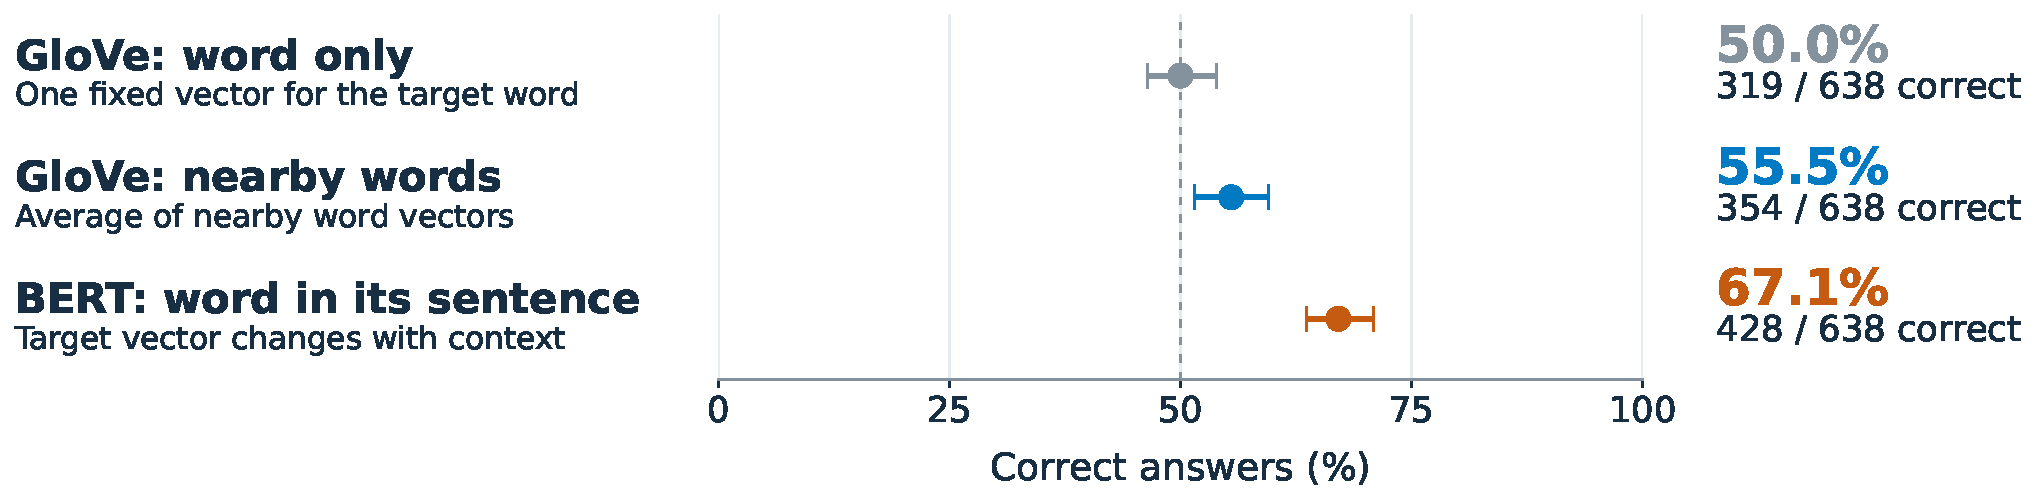
\includegraphics[width=\linewidth]{../../figures/poster_accuracy.pdf}
\end{minipage}\hfill
\begin{minipage}[c]{0.34\textwidth}\RaggedRight
{\fontsize{34}{40}\selectfont\bfseries\textcolor{accent}{+\AccuracyGain{} points}\par}
{\smallfont BERT over GloVe context. Paired 95\% interval: \GainLower{} to \GainUpper{} points. Layer \BestAccuracyLayer{} reaches 66.6\%, compared with 63.6\% at layer \FinalLayerNumber{}.}
\end{minipage}

\vfill
\ReferencesBlock
\end{document}
